\documentclass[10pt]{article}
\usepackage[utf8]{inputenc}
\usepackage[T1]{fontenc}
\usepackage{lmodern}
\usepackage[margin=1in]{geometry}
\usepackage{microtype}
\usepackage{booktabs}
\usepackage{tabularx}
\usepackage{array}
\usepackage{float}
\usepackage{tikz}
\usetikzlibrary{positioning,arrows.meta}
\usepackage[hidelinks]{hyperref}
\usepackage{cite}
\title{SafeOCR: Evidence-Grounded Selective Verification for Clinical OCR with Provenance-Preserving FHIR Export}
\author{Abdulaziz M. Alshehri, MPH\\Independent Researcher\\ORCID: \href{https://orcid.org/0009-0008-0536-5136}{0009-0008-0536-5136}\\\texttt{azialshehri@gmail.com}}
\date{Preprint}
\begin{document}
\maketitle
\begin{abstract}

\textbf{Objective.}

We developed and evaluated SafeOCR, a healthcare-specific verification layer that permits structured export only when critical OCR fields satisfy explicit evidence gates.

\textbf{Materials and Methods.}

SafeOCR v0.1 combines PaddleOCR with second-engine Tesseract rereads, structural checks, perturbation consistency, numeric and unit validation, provenance, and fail-closed review states. We evaluated a frozen policy on 288 synthetic critical-field cases, transcription generalization on 328 ClinOCR-Bench evaluation documents, and an oracle-localised verifier-component study on 238 public laboratory-report images.

\textbf{Results.}

On SafeOCR-LabGold, primary OCR made 0/288 errors (95\% Wilson upper bound 1.316\%). SafeOCR accepted 209/288 fields with 0/209 errors (upper bound 1.805\%) while routing 79 correct fields to review; this endpoint therefore did not demonstrate a safety gain. On ClinOCR-Bench, PaddleOCR mean WER was 0.4769 versus 0.5589 for local Tesseract, but PaddleOCR had 57/328 runtime failures (17.4\%), concentrated in rotated and mixed subsets, and failures were scored as empty predictions. In the laboratory-report component study, all 1,850 eligible primary numeric readings were exact; 375/1,850 passed the component gates with 0/375 numeric errors. Post-outcome exploratory analysis found 38/375 passes (10.1\%) had an analyte or unit mismatch.

\textbf{Discussion.}

SafeOCR provides an artifact-bound selective-verification workflow, but the current safety endpoints contained no primary-OCR errors for its gates to intercept.

\textbf{Conclusion.}

The study demonstrates feasibility, auditability, and the operational cost of selective verification rather than a demonstrated reduction in accepted error.

\end{abstract}
\section{Background and Significance}

Scanned clinical documents remain common, and OCR can recover structured data from laboratory reports and legacy records \cite{ma2023labocr,li2024tabular,hsu2022scanned}. For downstream use, however, transcription accuracy alone is not enough. A decimal, sign, comparator, or unit error can change meaning, and a correctly read value is still wrong if it is linked to the wrong analyte, row, or patient. OCR confidence alone does not establish that a field is sufficiently supported for automated structured export.

Selective prediction offers a complementary framing: when the expected cost of error is high, a system may abstain rather than force a prediction on every case \cite{geifman2019selectivenet}. In clinical data abstraction, this trade-off can be useful when review is preferable to an incorrect automated result \cite{swaminathan2024selective}. Recent work has also explored statistical risk control and conformal verification for accepted extractions \cite{angelopoulos2025learntest,kim2025conformalEHR}.

Trustworthy downstream reuse also requires traceability. FHIR provides a standardized interoperability layer, and prior work has linked clinical text mining and provenance with FHIR-based exchange \cite{daumke2019fhir,margheri2020provenance}. Yet conformance and provenance do not by themselves show that an OCR-derived field was read correctly from the source pixels.

Recent systems further narrow the novelty space. Girda and Groza introduced deterministic source-grounded trust promotion for laboratory data using same-row evidence, provenance, and review retention \cite{girda2026review}. RAPTOR applies generative document AI to clinical referral processing \cite{abioye2025raptor}, while RAPTOR+ evaluates clinical field extraction together with source-image bounding-box grounding \cite{abioye2026raptorplus}. Verified-abstention OCR has also been reported outside the clinical laboratory setting \cite{benhmida2025ontology}. SafeOCR therefore does not claim novelty for OCR, grounding, abstention, provenance, or FHIR individually.

Against this background, SafeOCR asks a narrower systems question: can a fail-closed evidence contract be evaluated transparently through coverage, review burden, and failure modes? Because the current primary OCR baselines make no errors on the primary safety endpoints, this study cannot estimate how much error reduction is attributable to the gates.

This paper makes four contributions:

\begin{enumerate}
\item an evidence-bound clinical OCR data model in which structured fields retain source-page and source-region provenance;
\item a fail-closed selective verification policy with explicit VERIFIED\_AUTO, REVIEW\_REQUIRED, and ABSTAINED terminal states;
\item a provenance-preserving FHIR R4 export gate that permits automated export only after verification;
\item a prespecified, commit-timestamped evaluation framework that reports accepted error jointly with verified coverage and preserves calibration/final-evaluation separation.
\end{enumerate}

Accordingly, SafeOCR is a systems-and-evaluation contribution rather than a claim of novelty for OCR, gating, abstention, provenance, or FHIR. Its narrower contribution is an artifact-bound specification and evaluation of a healthcare OCR verification contract that combines source evidence, second-engine rereading, perturbation stability, linkage and structure gates, criticality, selective decisions, and gated FHIR export \cite{girda2026review}.

\subsection{Related Work}

Clinical OCR studies show that scanned reports can be digitized but remain sensitive to layout and image quality \cite{ma2023labocr,li2024tabular,hsu2022scanned}. Recent laboratory/report systems extend layout-aware extraction and multimodal document understanding \cite{ren2025serialization,schafer2025transfusion}, while ClinOCR-Bench, MedStruct-S, Key Coverage Matters, and MedRepBench broaden evaluation across OCR artifacts, heterogeneous keys, and structured report interpretation \cite{hsu2026clinocr,li2026medstructs,wang2026keycoverage,shang2026medrepbench}.

SafeOCR's components also have clear prior art. Selective prediction and abstention formalize coverage-versus-error trade-offs and have been applied to clinical abstraction \cite{geifman2019selectivenet,swaminathan2024selective}; Learn-then-Test and conformal verification provide stronger risk-control frameworks that SafeOCR v0.1 does not claim \cite{angelopoulos2025learntest,kim2025conformalEHR}. Source-grounded admission for laboratory data, clinical document AI with review mechanisms, visual grounding, and verified-abstention OCR further narrow the novelty space \cite{girda2026review,abioye2025raptor,abioye2026raptorplus,benhmida2025ontology}. FHIR/text-mining and printed-form transformation work establish extraction-to-FHIR as prior art, while healthcare provenance work motivates auditable lineage \cite{daumke2019fhir,miller2023smarttext2fhir,werlitz2025printedfhir,margheri2020provenance}. SafeOCR therefore claims an integrated verification-and-evaluation contract, not novelty for OCR, grounding, abstention, provenance, or FHIR individually.

\section{Materials and Methods}

\subsection{Scope and safety boundary}

SafeOCR v0.1 was developed as research software for laboratory-report OCR verification. It is not a medical device or a clinical decision-support system. Medication documents, free-form handwritten notes, image interpretation, and automatic correction of clinically implausible text are outside its scope. Public evaluation is local-first and PHI-free.

\subsection{System architecture}
\begin{figure*}[t]
\centering
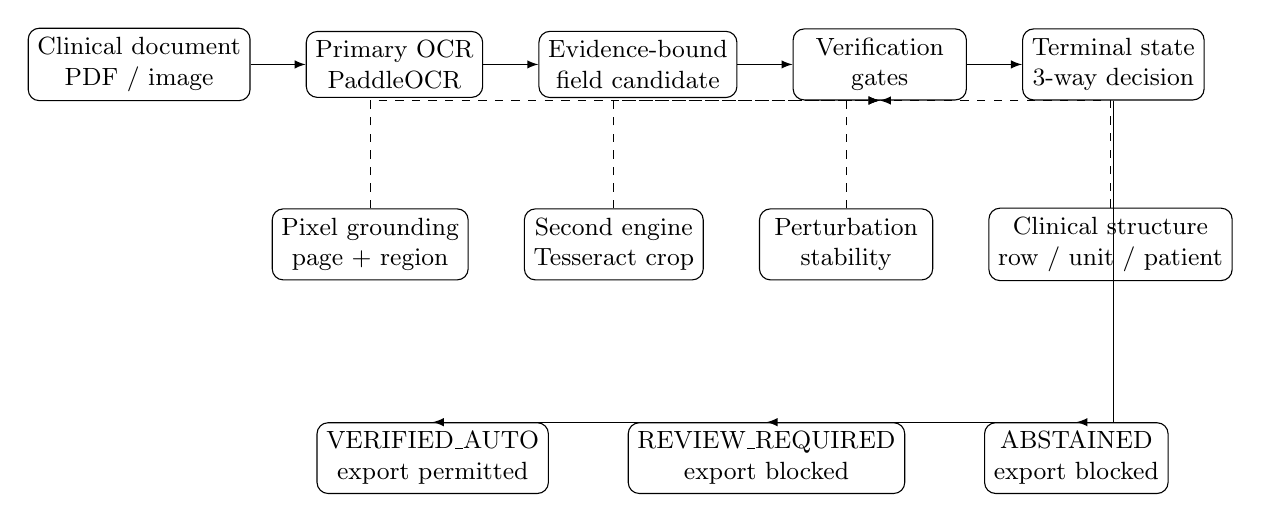
\begin{tikzpicture}[>=latex,node distance=7mm and 7mm,every node/.style={font=\small},box/.style={draw,rounded corners,align=center,minimum width=2.2cm,minimum height=0.82cm}]
\node[box] (doc) {Clinical document\\PDF / image};
\node[box,right=of doc] (ocr) {Primary OCR\\PaddleOCR};
\node[box,right=of ocr] (cand) {Evidence-bound\\field candidate};
\node[box,right=of cand] (gate) {Verification\\gates};
\node[box,right=of gate] (state) {Terminal state\\3-way decision};
\draw[->] (doc)--(ocr); \draw[->] (ocr)--(cand); \draw[->] (cand)--(gate); \draw[->] (gate)--(state);
\node[box,below=14mm of cand,xshift=-3.4cm] (g1) {Pixel grounding\\page + region};
\node[box,right=of g1] (g2) {Second engine\\Tesseract crop};
\node[box,right=of g2] (g3) {Perturbation\\stability};
\node[box,right=of g3] (g4) {Clinical structure\\row / unit / patient};
\foreach \g in {g1,g2,g3,g4}{\draw[dashed,->] (\g.north) |- (gate.south);}
\node[box,below=18mm of g2,xshift=-2.3cm] (v) {VERIFIED\_AUTO\\export permitted};
\node[box,right=10mm of v] (rev) {REVIEW\_REQUIRED\\export blocked};
\node[box,right=10mm of rev] (abs) {ABSTAINED\\export blocked};
\draw[->] (state.south) |- (v.north);
\draw[->] (state.south) |- (rev.north);
\draw[->] (state.south) |- (abs.north);
\end{tikzpicture}
\caption{SafeOCR v0.1 verification contract. Only VERIFIED\_AUTO fields may cross the automated structured-export boundary.}
\label{fig:architecture}
\end{figure*}

The pipeline is:

\begin{enumerate}
\item immutable document/page ingestion;
\item primary OCR and layout proposal;
\item construction of evidence-bound clinical field candidates;
\item second-engine critical-crop re-reading;
\item deterministic verification signals;
\item terminal decision: VERIFIED\_AUTO, REVIEW\_REQUIRED, or ABSTAINED;
\item FHIR R4 export only for VERIFIED\_AUTO fields;
\item static evidence report with source crop, decision reason, and provenance.
\end{enumerate}

PaddleOCR 3.7.0 is the primary full-page OCR path. Tesseract 5.4.0.20240606 is used as a second-engine critical-crop rereader and classical baseline.

\subsection{Evidence-bound field representation}

Each page is hash-bound, and each OCR span records the engine identity, page, bounding box, text, and native confidence when available. Structured laboratory fields retain the analyte, value, unit, source spans, association, criticality, and patient/document linkage. The EvidenceRecord stores the verification signals, policy version, terminal decision, failed gates, and recoverable source evidence. Correctness includes association: a correctly read number is still incorrect if it is linked to the wrong analyte, unit, row, date, or patient.

\subsection{Criticality}

The policy treats laboratory values, units, sign/decimal/comparator semantics, patient linkage, and meaning-changing row/column associations as critical; analyte identity, specimen/date/time, reference range, and abnormal flags are high criticality. Criticality changes verification strictness but never rewrites source text.

\subsection{Verification signals}

Automatic verification requires all mandatory gates: recoverable page/region grounding; unambiguous analyte-value-unit structure; Tesseract second-engine agreement on the primary-defined critical crop; stability of that reread under four frozen mild perturbations; unambiguous numeric parsing; valid unit syntax; unambiguous patient/document linkage; and healthy runtime execution. The second-engine and perturbation signals share the same primary-defined crop and are not statistically independent. Unit knowledge may veto export but never rewrite source text, and engine-native confidence is not treated as a calibrated probability.

\subsection{Decision states}

Each candidate reaches exactly one terminal state. \textbf{VERIFIED\_AUTO} means every required gate passed and automated export is permitted. \textbf{REVIEW\_REQUIRED} means the candidate is plausible but the evidence is insufficient or inconsistent. \textbf{ABSTAINED} means no reliable value could be established. REVIEW\_REQUIRED and ABSTAINED never fall back to automatic verification.

\subsection{FHIR R4 export gate}

Only VERIFIED\_AUTO fields may enter the FHIR export path. The export artifact includes provenance linking the structured resource back to source-document evidence. v0.1 targets FHIR R4 (4.0.1) \cite{hl7fhirr4}.

The FHIR runtime gate used HL7 validator CLI 6.10.4 against FHIR R4 (4.0.1) \cite{hl7fhirr4}. The single canonical valid bundle passed with zero validator errors; a deliberately invalid control was rejected with two errors. The validator produced seven warnings and one note on the valid bundle. Terminology validation was not evaluated as a clinical correctness endpoint. These results demonstrate structural/conformance validation only, not extraction correctness.

\subsection{Evaluation contract}

The evaluation contract was prespecified in version-controlled, commit-timestamped protocols rather than an external registry. Calibration and final evaluation are mechanically separated, so final outcomes cannot enter a tuning path. Primary reporting includes Critical Field Exact Accuracy, unsafe accepted error, verified coverage, review/abstention rates, and patient-attribution, table-association, or FHIR-mapping error only where estimable. Field-level 95\% Wilson intervals are descriptive: they do not model clustering or paired acquisitions, are not distribution-free guarantees, and zero observed errors never means zero underlying risk.

\subsection{SafeOCR-LabGold}

The frozen SafeOCR-LabGold final split contains 48 documents and 288 critical-field cases: 24 synthetic records, each rendered as a clean/corrupted pair across three templates (classic, compact, and grid), with six critical fields per document. The split hash was frozen before execution, and the primary final run was executed from a clean exact source head after calibration and qualification. Legacy per-field metrics use benchmark truth geometry only to align OCR spans with known field regions for scoring; they are not end-to-end field-discovery metrics. The separate table-association scorer uses OCR geometry only.

The compared operating points were:

\begin{itemize}
\item raw primary OCR;
\item Tesseract critical-crop reading;
\item naive exact agreement;
\item SafeOCR verification policy.
\end{itemize}

The primary v0.1 SafeOCR policy has one frozen operating point. We do not retrospectively sweep thresholds on the final set.

\subsection{External OCR generalization}

ClinOCR-Bench was used as a synthetic, template-generated, PHI-free benchmark of clinical-document OCR. Its release contains 384 documents: 56 exemplars and 328 evaluation documents spanning normal, handwriting, poor-quality, rotated, table, and mixed-artifact subsets \cite{hsu2026clinocr}. Before inspecting outcomes, we froze a no-tuning protocol for the two OCR engines already used by SafeOCR. Ground-truth transcripts were unavailable to the OCR runner and were opened only by a separate scorer after all predictions had been written. Word error rate (WER), substitutions, deletions, and insertions were calculated using whitespace tokenization compatible with the official ClinOCR-Bench baseline implementation.

The external experiment evaluates transcription generalization only. ClinOCR-Bench v1.0 provides full-document transcript ground truth rather than the field, patient-linkage, association, and FHIR annotations required for SafeOCR safety endpoints; therefore document-level WER is not converted into unsafe-accept or verified-coverage claims.

\subsection{External laboratory-report verifier-component evaluation}

We used the public laboratory-report image collection released by Xue et al. and subsequently used and described by Ma et al. \cite{xue2020labocr,ma2023labocr}. Ma et al. describe 238 de-identified Chinese laboratory-report images derived from 119 paper reports and captured by scanners and smartphones under varied illumination. Their reported dual-annotation Cohen's kappa of 0.89 applies to the separate PKU1 dataset, not to this public image collection; the provenance of the public collection's text/cell labels is not documented in the source materials available to this study. Before scoring, frozen PaddleOCR inference was executed on all 238 images with the annotation source inaccessible to the OCR runner; no OCR runtime failures occurred.

Gold annotations were opened only after OCR to identify analyte, numeric-value, and unit regions for an \textbf{oracle-localised verifier-component evaluation}. They were not used to generate OCR predictions, choose preprocessing, tune thresholds, or locate regions during OCR inference. Scoring used laboratory table 2, excluding the header row, and aligned OCR spans to gold cells only after OCR with a minimum truth-area overlap of 0.25; candidates were ranked by overlap and then OCR confidence. Eligible rows required non-empty analyte, value, and unit annotations plus a parseable numeric value. Duplicate annotations in the estimand-relevant analyte/value/unit cells were excluded fail-closed rather than arbitrarily adjudicated.

A component pass required visual grounding, second-engine Tesseract agreement on the numeric-value crop, stability across the four frozen perturbations, structural association, successful numeric parsing, and valid unit syntax. The primary external component endpoint was prespecified in code before outcome generation as an incorrect numeric value among component-passed fields (commit 47433ae8fb429671489ac530dfd05c95a82bfaf4; the result was frozen later at commit 6f082d8dad6d576c8add7a5914609c68785ef665). This endpoint is narrower than the paper's general full-field correctness definition and does not test end-to-end field discovery, analyte semantic verification, patient linkage, the complete VERIFIED\_AUTO policy, or FHIR mapping.

\section{Results}

\subsection{Primary final evaluation}
\begin{figure}[H]
\centering
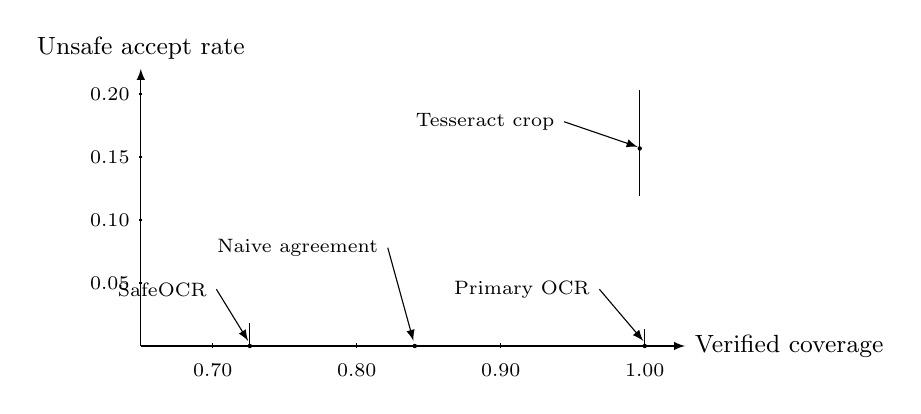
\begin{tikzpicture}[x=6.4cm,y=16cm,>=latex]
% Coverage axis is rescaled from 0.65--1.00 to plot coordinates 0--1.
\draw[->] (0,0)--(1.08,0) node[right]{\small Verified coverage};
\draw[->] (0,0)--(0,0.22) node[above]{\small Unsafe accept rate};

% x_plot = (coverage - 0.65) / 0.35.
\foreach \x/\lab in {0.1429/0.70,0.4286/0.80,0.7143/0.90,1.0000/1.00}{
  \draw (\x,0.002)--(\x,-0.002) node[below,yshift=-2pt]{\scriptsize \lab};
}
\foreach \y/\lab in {0.05/0.05,0.10/0.10,0.15/0.15,0.20/0.20}{
  \draw (0.003,\y)--(-0.003,\y) node[left]{\scriptsize \lab};
}

% SafeOCR: coverage 0.7257 -> x=0.2163.
\draw (0.2163,0)--(0.2163,0.01805);
\fill (0.2163,0) circle (0.8pt);
\node[anchor=east] (safeLabel) at (0.15,0.045){\scriptsize SafeOCR};
\draw[thin,->] (safeLabel.east)--(0.213,0.004);

% Naive agreement: coverage 0.8403 -> x=0.5437.
\fill (0.5437,0) circle (0.8pt);
\node[anchor=east] (naiveLabel) at (0.49,0.078){\scriptsize Naive agreement};
\draw[thin,->] (naiveLabel.east)--(0.541,0.004);

% Primary OCR: coverage 1.0 -> x=1.0.
\draw (1,0)--(1,0.01316);
\fill (1,0) circle (0.8pt);
\node[anchor=east] (primaryLabel) at (0.91,0.045){\scriptsize Primary OCR};
\draw[thin,->] (primaryLabel.east)--(0.997,0.004);

% Tesseract crop: coverage 0.9965 -> x=0.9900.
\draw (0.9900,0.1193)--(0.9900,0.2034);
\fill (0.9900,0.1568) circle (0.8pt);
\node[anchor=east] (tessLabel) at (0.84,0.178){\scriptsize Tesseract crop};
\draw[thin,->] (tessLabel.east)--(0.986,0.158);
\end{tikzpicture}
\caption{Frozen LabGold operating points. The primary OCR baseline had no errors, so the zero-event gated result does not demonstrate a safety gain. Vertical bars are descriptive 95\% Wilson intervals.}
\label{fig:riskcoverage}
\end{figure}

The frozen final set contained 288 evaluable critical-field cases.

\begin{table*}[t]
\centering\small
\caption{Frozen SafeOCR-LabGold operating points.}
\label{tab:labgold}
\begin{tabularx}{\textwidth}{>{\raggedright\arraybackslash}X>{\raggedright\arraybackslash}X>{\raggedright\arraybackslash}X>{\raggedright\arraybackslash}X>{\raggedright\arraybackslash}X>{\raggedright\arraybackslash}X>{\raggedright\arraybackslash}X}
\toprule
Method & Accepted & Review & Abstain & Verified coverage & Unsafe accepts & Unsafe accept rate \\
\midrule
Primary OCR & 288 & 0 & 0 & 100.00\% & 0 & 0.00\% observed \\
Tesseract crop & 287 & 0 & 1 & 99.65\% & 45 & 15.68\% \\
Naive agreement & 242 & 46 & 0 & 84.03\% & 0 & 0.00\% observed \\
SafeOCR & 209 & 79 & 0 & 72.57\% & 0 & 0.00\% observed \\
\bottomrule
\end{tabularx}
\end{table*}

SafeOCR accepted 209 fields and routed 79 to review. No unsafe accepts were observed among the accepted fields; the 95\% Wilson interval was 0 to 0.01805. Raw primary OCR, however, also made 0/288 errors at full coverage, with a tighter 95\% Wilson upper bound of 0.01316. All 79 reviewed fields were therefore correct under benchmark truth, leaving no endpoint errors for the verification gate to intercept. This result measures feasibility and review cost rather than a demonstrated safety gain over the primary OCR baseline.

The Tesseract crop baseline produced 45 unsafe accepts among 287 accepted fields, corresponding to an unsafe accept rate of 0.1568 (95\% Wilson interval approximately 0.1193-0.2034).

As a post-outcome descriptive dependence sensitivity, 0/48 LabGold documents and 0/24 underlying clean/corrupt record pairs contained any primary-OCR field error; corresponding Wilson upper bounds are 7.41\% and 13.80\%, respectively. These coarser bounds are not substitutes for a prespecified cluster-aware analysis but illustrate how field-level uncertainty understates dependence.

\subsection{Table association}

A separate OCR-geometry-only association scorer evaluated 288/288 cases and observed zero table-association errors. The scorer did not use truth geometry to parse rows. This result is limited to the synthetic LabGold structure and should not be generalized to arbitrary real-world report layouts.

\subsection{FHIR validator evidence}

The canonical FHIR R4 bundle passed HL7 validator CLI 6.10.4 with zero errors. Seven warnings and one note were recorded. A deliberately invalid control was rejected with two errors.

This shows that the tested export artifact satisfied the validator gate. It does not provide a benchmark estimate of clinical FHIR mapping correctness because per-field FHIR mapping error was not included in the prespecified, commit-timestamped F6 final run.

\subsection{Evidence traceability}

The static evidence artifact illustrates field-level traceability for one verified laboratory value. The example includes source-page SHA-256, bounding boxes for analyte/value/unit spans, OCR engine/version, policy version, verification signals, decision state, failed gates, and a deterministic explanation. The corresponding source crop is hash-bound.

\subsection{External OCR generalization on ClinOCR-Bench}

Both frozen OCR engines were scored across all 328 ClinOCR-Bench evaluation documents under the frozen failure policy. Local Tesseract produced a mean WER of 0.5589 (95\% CI 0.5209-0.5968) and median WER of 0.5647. Frozen PaddleOCR produced a mean WER of 0.4769 (95\% CI 0.4372-0.5165) and median WER of 0.3659, but it incurred 57/328 runtime failures (17.4\%): 33/56 rotated documents and 24/48 mixed-artifact documents. Under the frozen failure policy, these failures were retained in the denominator and scored as empty predictions.

Performance varied substantially by artifact type. PaddleOCR mean WER was 0.1149 on normal documents, 0.2694 on poor-quality documents, 0.2847 on tables, 0.4256 on handwriting, 0.9035 on rotated documents, and 0.9276 on mixed-artifact documents. Tesseract similarly showed strong artifact sensitivity, with mean WER ranging from 0.1089 on normal documents to 0.9225 on mixed-artifact documents. Across all 328 paired documents, the descriptive mean PaddleOCR-minus-Tesseract WER difference was -0.0820 (fixed-seed paired bootstrap 95\% interval -0.1204 to -0.0442). In a labelled sensitivity restricted to the 271 documents without a PaddleOCR runtime failure, PaddleOCR mean WER was 0.3668 versus 0.5358 for Tesseract; on the 57 PaddleOCR-failure documents, Tesseract mean WER was 0.6686. These analyses are descriptive and do not alter the frozen failure policy or primary benchmark results.

The prespecified official-versus-local Tesseract comparison (Table 2) showed the largest discrepancy on rotation (median WER 1.0000 vs 0.5802), preventing treatment of the local run as an exact reproduction of the authors' environment.

\begin{table*}[t]
\centering\small
\caption{Official ClinOCR-Bench versus local frozen Tesseract median word error rate.}
\label{tab:clinocr-tess}
\begin{tabularx}{\textwidth}{>{\raggedright\arraybackslash}X>{\raggedright\arraybackslash}X>{\raggedright\arraybackslash}X}
\toprule
ClinOCR subset & Official Tesseract median WER & Local frozen Tesseract median WER \\
\midrule
Normal & 0.0866 & 0.1099 \\
Handwriting & 0.8228 & 0.8135 \\
Poor quality & 0.8184 & 0.8205 \\
Rotation & 1.0000 & 0.5802 \\
Tables & 0.4578 & 0.3244 \\
Mixed & 1.0000 & 0.9846 \\
\bottomrule
\end{tabularx}
\end{table*}

These results are transcription-generalization evidence only. ClinOCR-Bench is synthetic and not laboratory-report-specific, and the SafeOCR verification contract is not exercised on it. The failure concentration in rotated and mixed documents is therefore interpreted as a fail-closed engineering finding rather than field-level clinical safety evidence.

\subsection{External verifier-component evaluation on public laboratory reports}

The public laboratory-report dataset yielded 1,850 eligible analyte-value-unit rows from 2,219 candidate laboratory rows after frozen eligibility and annotation-integrity rules. Exclusions were 275 unsupported gold values, 74 missing units, 13 ambiguous duplicate rows, 4 missing values, and 3 missing analytes. Eligible rows came from 180/238 images; 58 images contributed no eligible row under the frozen table/eligibility rules.

\begin{table*}[t]
\centering\small
\caption{External laboratory-report cohort flow under frozen eligibility rules.}
\label{tab:cohort}
\begin{tabularx}{\textwidth}{>{\raggedright\arraybackslash}X>{\raggedright\arraybackslash}X}
\toprule
Ma2023 cohort step & Rows \\
\midrule
Candidate laboratory rows & 2,219 \\
Excluded: unsupported gold value & 275 \\
Excluded: missing unit & 74 \\
Excluded: ambiguous duplicate critical cell & 13 \\
Excluded: missing value & 4 \\
Excluded: missing analyte & 3 \\
Eligible rows & 1,850 \\
\bottomrule
\end{tabularx}
\end{table*}

The primary value span was localised in 1,850/1,850 cases and the complete analyte/value/unit context in 1,849/1,850. Primary OCR reproduced the annotated numeric value in all 1,850 eligible cases, while the complete analyte-value-unit tuple was exact in 1,461/1,850 (78.97\%).

The component gates passed 375/1,850 fields (20.27\%). Second-engine numeric-value agreement passed in 654/1,850 (35.35\%), perturbation stability in 449/1,850 (24.27\%), structural association in 1,837/1,850 (99.30\%), and unit validation in 1,347/1,850 (72.81\%). The overlapping gate funnel was 654 with second-engine agreement, 442 with both agreement and perturbation stability, 377 after additionally requiring valid unit syntax, and 375 after additionally requiring structural association.

\begin{table*}[t]
\centering\small
\caption{Overlapping verifier-component gate funnel.}
\label{tab:funnel}
\begin{tabularx}{\textwidth}{>{\raggedright\arraybackslash}X>{\raggedright\arraybackslash}X>{\raggedright\arraybackslash}X}
\toprule
Frozen component funnel & Rows & Coverage \\
\midrule
Eligible & 1,850 & 100.00\% \\
Second-engine agreement & 654 & 35.35\% \\
Agreement + perturbation stability & 442 & 23.89\% \\
+ valid unit syntax & 377 & 20.38\% \\
+ structural association / component pass & 375 & 20.27\% \\
\bottomrule
\end{tabularx}
\end{table*}

No runtime failures occurred. No component-passed field contained an incorrect numeric value (0/375; observed rate 0\%, 95\% Wilson interval 0-1.014\%), but the ungated primary numeric reading was also exact in 1,850/1,850 rows (95\% Wilson upper bound 0.207\%). Therefore the numeric endpoint contained no primary-OCR errors for the component gates to intercept; all 1,475 rejected numeric values were correct under the frozen reference labels.

Component-pass coverage was similar for scanner images (192/926; 20.73\%) and illumination/smartphone variants (183/924; 19.81\%). In contrast, complete primary field exactness fell from 814/926 (87.90\%) on scans to 647/924 (70.02\%) under illumination variants.

As a post-outcome descriptive cluster sensitivity, the 375 component passes arose from 86 images, and 0/86 of those images contained an incorrect accepted numeric value; the Wilson upper bound at the image-event level is 4.28\%. This does not redefine the field-level endpoint or provide a population-level guarantee.

A prespecified primary claim is not made for full field-tuple correctness among component passes because the frozen component endpoint concerns the numeric value. A separately labelled post-outcome diagnostic found that 38/375 passed fields (10.13\%; 95\% Wilson interval 7.47\%-13.60\%) had an analyte or unit mismatch: 36 analyte mismatches and 2 unit mismatches, with no numeric-value mismatches. Equivalently, 337/375 tuples were exact. This exploratory diagnostic is given equal prominence because it exposes the narrower scope of numeric verification; it does not alter the frozen primary component endpoint.

\section{Discussion}

\subsection{Principal findings}

SafeOCR makes acceptance explicit and auditable: fields are source-bound, checked by a second OCR engine and structural rules, routed to VERIFIED\_AUTO, REVIEW\_REQUIRED, or ABSTAINED, and only verified fields may enter automated FHIR export. The frozen LabGold policy accepted 72.57\% of fields, but primary OCR was already correct in 288/288 cases. The 79 reviews therefore intercepted no endpoint error. The result measures implementation feasibility and review cost, not safety improvement.

The external studies reinforce this boundary. ClinOCR-Bench exposed substantial transcription and runtime brittleness, including 57/328 PaddleOCR failures, but it does not exercise SafeOCR's field-level contract. In the public laboratory-report component study, primary numeric OCR was exact in 1,850/1,850 eligible rows, so the 375 component passes likewise could not demonstrate numeric error reduction. More informative was the exploratory finding that 38/375 component passes had an analyte or unit mismatch, showing that numeric agreement does not establish full-field correctness.

\subsection{Relation to selective verification and risk control}

SafeOCR follows the selective-prediction principle that abstention/review can be preferable to forced prediction \cite{swaminathan2024selective,geifman2019selectivenet}, but uses deterministic evidence gates rather than a learned reject function. Its explicit failure reasons improve inspectability, at the cost of substantial rejected coverage. Unlike formal risk-control approaches \cite{angelopoulos2025learntest,kim2025conformalEHR}, v0.1 provides no conformal or distribution-free guarantee; its uncertainty intervals are descriptive.

\subsection{Provenance and interoperability}

In SafeOCR, source-region provenance is part of the acceptance contract rather than a retrospective log: a critical field without recoverable source evidence cannot reach VERIFIED\_AUTO. FHIR remains an export boundary, not evidence that extraction was correct. This distinction separates source verification from interoperability and validator conformance \cite{daumke2019fhir,hl7fhirr4}.

\subsection{External validity and design implications}

ClinOCR-Bench is synthetic and transcript-level; proper external SafeOCR validation requires prediction-blind field identity, value, unit, association, and source-region truth. The public Xue/Ma study adds real report images but remains oracle-localised and has undocumented label-generation provenance. Its 10.1\% exploratory tuple-mismatch rate motivates second-engine verification of analyte identity and unit semantics, not only numeric crops. Future studies should be end-to-end, prespecified, cluster-aware, independently adjudicated, and include data on which primary OCR makes measurable full-tuple errors.

\subsection{Limitations}

First, LabGold is synthetic (24 records, paired clean/corrupt renderings, three templates), uses truth geometry for legacy per-field score alignment, and had zero primary-OCR errors; it therefore cannot establish a gating benefit or end-to-end field discovery performance. ABSTAINED was not exercised.

Second, ClinOCR-Bench is synthetic, not laboratory-specific, and evaluates transcription rather than the verification contract. Its field-level confidence intervals ignore template clustering, and the local Tesseract environment differs materially from the official baseline on rotation.

Third, the Xue/Ma experiment is oracle-localised. Public label-generation provenance is undocumented; modern OCR training-set contamination cannot be excluded; 58/238 images contributed no eligible row; and the implemented scorer required non-empty units for the whole component estimand although the frozen prose protocol limited that rule to unit-dependent analysis. Three pre-outcome repairs—JPEG-to-PNG normalization, page-identity rebinding, and fail-closed exclusion of 13 ambiguous duplicate rows—occurred before any result artifact existed. Patient linkage, full VERIFIED\_AUTO behavior, and FHIR mapping were not evaluated, and tuple mismatch analysis is post-outcome exploratory.

Fourth, field-level Wilson intervals do not model dependence within LabGold record pairs or external images; cluster sensitivities are descriptive only. FHIR evidence is a single-bundle validator smoke test plus invalid control, without terminology or mapping-accuracy evaluation. The traceability artifact is one example, not a human-factors study. Finally, the work does not evaluate diagnosis, treatment, deployment safety, or medical-device performance.

\subsection{Future Work}

Priority next steps are a separately prespecified end-to-end study with non-zero baseline full-tuple errors; independently adjudicated multi-institution validation; verification of analyte, unit, and patient linkage; formal risk-control calibration; and prospective review studies measuring correction burden and FHIR mapping correctness.

\section{Conclusion}

Clinical OCR should not be evaluated only as a transcription problem when its output is intended for structured healthcare data. SafeOCR specifies and evaluates a field-level verification contract that connects evidence binding, second-engine checks, explicit review or abstention, and provenance-preserving FHIR export in a fail-closed pipeline.

On the frozen v0.1 synthetic evaluation, SafeOCR automatically verified 72.57\% of critical fields, but the primary OCR baseline also produced zero observed errors and all 79 reviewed fields were correct under benchmark truth. In the oracle-localised public laboratory-report evaluation, the primary numeric reading was exact in all 1,850 eligible rows, so the 0/375 numeric-error result among component passes could not demonstrate a safety gain. Exploratory analysis instead found analyte or unit mismatches in 38/375 passes. The appropriate conclusion is not that SafeOCR is safer, superior, or clinically validated, but that an evidence-gated workflow can be implemented and audited at a substantial coverage cost. Future prespecified evaluation must include genuine primary-OCR errors and verification beyond numeric values.

\section*{Data and Code Availability}

SafeOCR source code, frozen protocols, scoring code, and derived evidence artifacts are released under the repository's Apache-2.0 software license where applicable. SafeOCR-LabGold is synthetic and ClinOCR-Bench is public and PHI-free. The public laboratory-report images originate from Xue et al.'s repository and are not redistributed by SafeOCR. No dataset-wide license file was identified in the audited upstream repository state; users should obtain the images from the original source and determine permitted reuse under the publication and repository terms applicable to them.

\section*{Ethics and Safety Statement}

SafeOCR-LabGold is synthetic and ClinOCR-Bench is PHI-free. The external laboratory-report analysis uses a public image collection described by Ma et al. as de-identified and originally released with Xue et al.'s work; SafeOCR does not redistribute those source images. This study involved no new participant recruitment, intervention, or access to identifiable patient data. SafeOCR is research software and is not intended for diagnosis, treatment decisions, or unsupervised clinical use. Any journal-specific institutional-review statement will be limited to a determination actually obtained or required for the author's jurisdiction and affiliation.

\section*{Funding}

This research received no external funding.

\section*{Competing Interests}

The author declares no competing interests.

\section*{Research tools}

\textbf{Research tools:} Google NotebookLM was used for literature-search support, Zotero for reference management, and Perplexity for deep-search support.

\bibliographystyle{unsrt}
\bibliography{references}
\end{document}
